
\section{Fuchsjagd (ARDF)}
\label{section:ardf}
\begin{frame}%STARTCONTENT

\frametitle{Fuchsjagd (ARDF)}
\begin{itemize}
  \item Eine weitere Art von Wettbewerb ist das Amateur Radio Direction Finding (ARDF).
  \item Die „Füchse“ sind kleine versteckte Sender, die von den Teilnehmern mittels Peilempfängern gefunden und zu Fuß angelaufen werden müssen.
  \item Die Füchse senden im zeitlichem Wechsel jeweils ein anderes der folgende Rufzeichen in CW-Morsetelegrafie aus: MO, MOE, MOI, MOS, MOH oder MO5.
  \end{itemize}
\end{frame}

\begin{frame}
\frametitle{Rufzeichen der Fuchsjagdsender}
\begin{columns}
    \begin{column}{0.48\textwidth}
    \begin{table}
\begin{DARCtabular}{ll}
     Rufzeichen  & Morse-Code   \\
     MO  & \MorseDah\MorseDah\MorseCharSep\MorseDah\MorseDah\MorseDah   \\
     MOE  & \MorseDah\MorseDah\MorseCharSep\MorseDah\MorseDah\MorseDah\MorseCharSep\MorseDit   \\
     MOI  & \MorseDah\MorseDah\MorseCharSep\MorseDah\MorseDah\MorseDah\MorseCharSep\MorseDit\MorseDit   \\
     MOS  & \MorseDah\MorseDah\MorseCharSep\MorseDah\MorseDah\MorseDah\MorseCharSep\MorseDit\MorseDit\MorseDit   \\
     MOH  & \MorseDah\MorseDah\MorseCharSep\MorseDah\MorseDah\MorseDah\MorseCharSep\MorseDit\MorseDit\MorseDit\MorseDit   \\
     MO5  & \MorseDah\MorseDah\MorseCharSep\MorseDah\MorseDah\MorseDah\MorseCharSep\MorseDit\MorseDit\MorseDit\MorseDit\MorseDit   \\
\end{DARCtabular}
\caption{Rufzeichen der Fuchsjagdsender}
\label{ardf_morse_code}
\end{table}

    \end{column}
   \begin{column}{0.48\textwidth}
       
\begin{figure}
    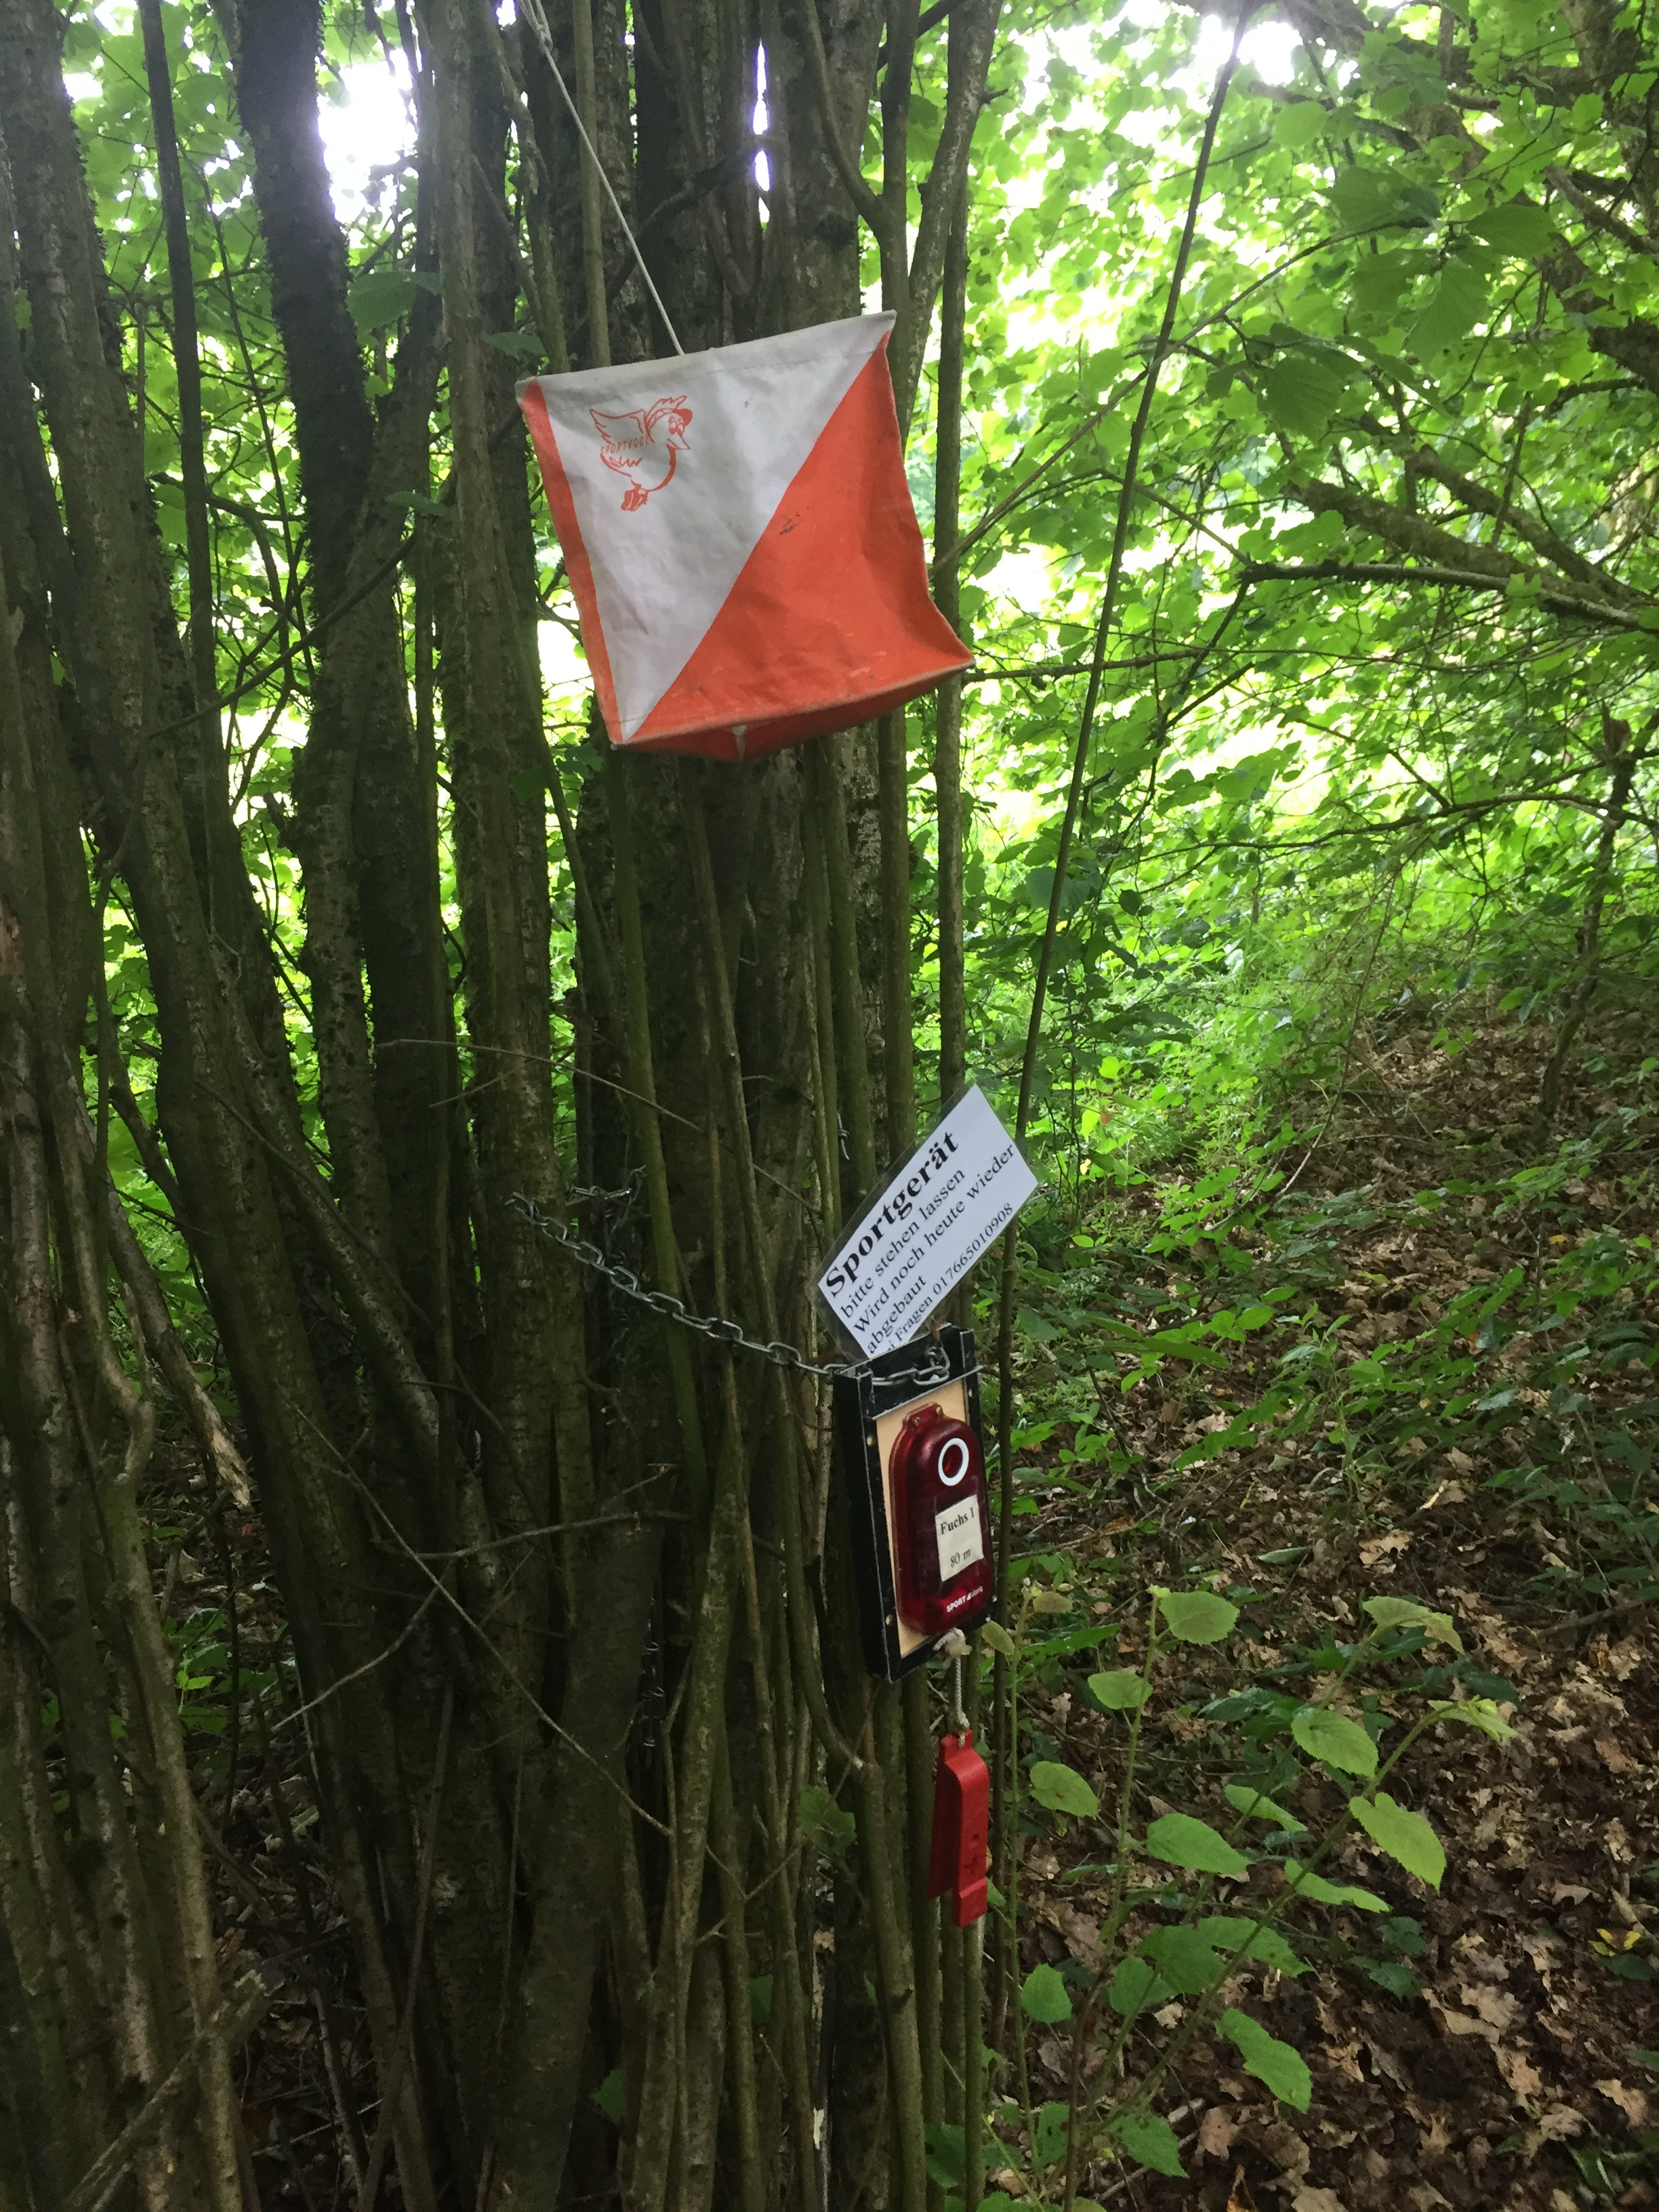
\includegraphics[width=0.85\textwidth]{foto/190}
    \caption{\scriptsize ARDF-Fuchs im Wald mit Wimpel und Zeitnehmer}
    \label{n_ardf_fuchs}
\end{figure}

   \end{column}
\end{columns}

\end{frame}

\begin{frame}
\only<1>{
\begin{QQuestion}{BE313}{Was verstehen Funkamateure unter einer \glqq Fuchsjagd\grqq{} (ARDF = Amateur Radio Direction Finding)?}{Es ist ein Funkwettbewerb, wobei versucht wird, in einer vorgegebenen Zeit auf einem Amateurfunkband mit möglichst vielen Ländern Funkverbindungen herzustellen.}
{Es ist ein Funkpeilwettbewerb, wobei mit Hilfe von tragbaren Peilempfängern versteckte Kleinsender im KW- oder UKW-Bereich, die nur kurzzeitig senden, aufzufinden sind.}
{Bei der Fuchsjagd wird versucht, den Weg von mobilen Kleinsendern zu verfolgen und dabei ein Muster zu erkennen.}
{Es ist ein Funkpeilwettbewerb, der von Funkamateuren ausschließlich für SWL's (short wave listeners) veranstaltet wird. }
\end{QQuestion}

}
\only<2>{
\begin{QQuestion}{BE313}{Was verstehen Funkamateure unter einer \glqq Fuchsjagd\grqq{} (ARDF = Amateur Radio Direction Finding)?}{Es ist ein Funkwettbewerb, wobei versucht wird, in einer vorgegebenen Zeit auf einem Amateurfunkband mit möglichst vielen Ländern Funkverbindungen herzustellen.}
{\textbf{\textcolor{DARCgreen}{Es ist ein Funkpeilwettbewerb, wobei mit Hilfe von tragbaren Peilempfängern versteckte Kleinsender im KW- oder UKW-Bereich, die nur kurzzeitig senden, aufzufinden sind.}}}
{Bei der Fuchsjagd wird versucht, den Weg von mobilen Kleinsendern zu verfolgen und dabei ein Muster zu erkennen.}
{Es ist ein Funkpeilwettbewerb, der von Funkamateuren ausschließlich für SWL's (short wave listeners) veranstaltet wird. }
\end{QQuestion}

}
\end{frame}

\begin{frame}
\only<1>{
\begin{QQuestion}{BD109}{Welche Kennungen werden von leistungsschwachen Amateurfunksendern zu Peilzwecken ausgesendet?}{MO, MOE, MOI, MOS, MOH oder MO5}
{DO, DOE, DOI, DOS, DOH oder DO5}
{DL, DL1, DL2, DL3, DL4 oder DL5}
{ARDF, ARDF1, ARDF2, ARDF3, ARDF4 oder ARDF5}
\end{QQuestion}

}
\only<2>{
\begin{QQuestion}{BD109}{Welche Kennungen werden von leistungsschwachen Amateurfunksendern zu Peilzwecken ausgesendet?}{\textbf{\textcolor{DARCgreen}{MO, MOE, MOI, MOS, MOH oder MO5}}}
{DO, DOE, DOI, DOS, DOH oder DO5}
{DL, DL1, DL2, DL3, DL4 oder DL5}
{ARDF, ARDF1, ARDF2, ARDF3, ARDF4 oder ARDF5}
\end{QQuestion}

}
\end{frame}%ENDCONTENT
